% Options for packages loaded elsewhere
\PassOptionsToPackage{unicode}{hyperref}
\PassOptionsToPackage{hyphens}{url}
\PassOptionsToPackage{dvipsnames,svgnames,x11names}{xcolor}
%
\documentclass[
  letterpaper,
  DIV=11,
  numbers=noendperiod,
  oneside]{scrartcl}

\usepackage{amsmath,amssymb}
\usepackage{lmodern}
\usepackage{iftex}
\ifPDFTeX
  \usepackage[T1]{fontenc}
  \usepackage[utf8]{inputenc}
  \usepackage{textcomp} % provide euro and other symbols
\else % if luatex or xetex
  \usepackage{unicode-math}
  \defaultfontfeatures{Scale=MatchLowercase}
  \defaultfontfeatures[\rmfamily]{Ligatures=TeX,Scale=1}
\fi
% Use upquote if available, for straight quotes in verbatim environments
\IfFileExists{upquote.sty}{\usepackage{upquote}}{}
\IfFileExists{microtype.sty}{% use microtype if available
  \usepackage[]{microtype}
  \UseMicrotypeSet[protrusion]{basicmath} % disable protrusion for tt fonts
}{}
\makeatletter
\@ifundefined{KOMAClassName}{% if non-KOMA class
  \IfFileExists{parskip.sty}{%
    \usepackage{parskip}
  }{% else
    \setlength{\parindent}{0pt}
    \setlength{\parskip}{6pt plus 2pt minus 1pt}}
}{% if KOMA class
  \KOMAoptions{parskip=half}}
\makeatother
\usepackage{xcolor}
\usepackage[left=1in,marginparwidth=2.0666666666667in,textwidth=4.1333333333333in,marginparsep=0.3in]{geometry}
\setlength{\emergencystretch}{3em} % prevent overfull lines
\setcounter{secnumdepth}{5}
% Make \paragraph and \subparagraph free-standing
\ifx\paragraph\undefined\else
  \let\oldparagraph\paragraph
  \renewcommand{\paragraph}[1]{\oldparagraph{#1}\mbox{}}
\fi
\ifx\subparagraph\undefined\else
  \let\oldsubparagraph\subparagraph
  \renewcommand{\subparagraph}[1]{\oldsubparagraph{#1}\mbox{}}
\fi

\usepackage{color}
\usepackage{fancyvrb}
\newcommand{\VerbBar}{|}
\newcommand{\VERB}{\Verb[commandchars=\\\{\}]}
\DefineVerbatimEnvironment{Highlighting}{Verbatim}{commandchars=\\\{\}}
% Add ',fontsize=\small' for more characters per line
\usepackage{framed}
\definecolor{shadecolor}{RGB}{241,243,245}
\newenvironment{Shaded}{\begin{snugshade}}{\end{snugshade}}
\newcommand{\AlertTok}[1]{\textcolor[rgb]{0.68,0.00,0.00}{#1}}
\newcommand{\AnnotationTok}[1]{\textcolor[rgb]{0.37,0.37,0.37}{#1}}
\newcommand{\AttributeTok}[1]{\textcolor[rgb]{0.40,0.45,0.13}{#1}}
\newcommand{\BaseNTok}[1]{\textcolor[rgb]{0.68,0.00,0.00}{#1}}
\newcommand{\BuiltInTok}[1]{\textcolor[rgb]{0.00,0.23,0.31}{#1}}
\newcommand{\CharTok}[1]{\textcolor[rgb]{0.13,0.47,0.30}{#1}}
\newcommand{\CommentTok}[1]{\textcolor[rgb]{0.37,0.37,0.37}{#1}}
\newcommand{\CommentVarTok}[1]{\textcolor[rgb]{0.37,0.37,0.37}{\textit{#1}}}
\newcommand{\ConstantTok}[1]{\textcolor[rgb]{0.56,0.35,0.01}{#1}}
\newcommand{\ControlFlowTok}[1]{\textcolor[rgb]{0.00,0.23,0.31}{#1}}
\newcommand{\DataTypeTok}[1]{\textcolor[rgb]{0.68,0.00,0.00}{#1}}
\newcommand{\DecValTok}[1]{\textcolor[rgb]{0.68,0.00,0.00}{#1}}
\newcommand{\DocumentationTok}[1]{\textcolor[rgb]{0.37,0.37,0.37}{\textit{#1}}}
\newcommand{\ErrorTok}[1]{\textcolor[rgb]{0.68,0.00,0.00}{#1}}
\newcommand{\ExtensionTok}[1]{\textcolor[rgb]{0.00,0.23,0.31}{#1}}
\newcommand{\FloatTok}[1]{\textcolor[rgb]{0.68,0.00,0.00}{#1}}
\newcommand{\FunctionTok}[1]{\textcolor[rgb]{0.28,0.35,0.67}{#1}}
\newcommand{\ImportTok}[1]{\textcolor[rgb]{0.00,0.46,0.62}{#1}}
\newcommand{\InformationTok}[1]{\textcolor[rgb]{0.37,0.37,0.37}{#1}}
\newcommand{\KeywordTok}[1]{\textcolor[rgb]{0.00,0.23,0.31}{#1}}
\newcommand{\NormalTok}[1]{\textcolor[rgb]{0.00,0.23,0.31}{#1}}
\newcommand{\OperatorTok}[1]{\textcolor[rgb]{0.37,0.37,0.37}{#1}}
\newcommand{\OtherTok}[1]{\textcolor[rgb]{0.00,0.23,0.31}{#1}}
\newcommand{\PreprocessorTok}[1]{\textcolor[rgb]{0.68,0.00,0.00}{#1}}
\newcommand{\RegionMarkerTok}[1]{\textcolor[rgb]{0.00,0.23,0.31}{#1}}
\newcommand{\SpecialCharTok}[1]{\textcolor[rgb]{0.37,0.37,0.37}{#1}}
\newcommand{\SpecialStringTok}[1]{\textcolor[rgb]{0.13,0.47,0.30}{#1}}
\newcommand{\StringTok}[1]{\textcolor[rgb]{0.13,0.47,0.30}{#1}}
\newcommand{\VariableTok}[1]{\textcolor[rgb]{0.07,0.07,0.07}{#1}}
\newcommand{\VerbatimStringTok}[1]{\textcolor[rgb]{0.13,0.47,0.30}{#1}}
\newcommand{\WarningTok}[1]{\textcolor[rgb]{0.37,0.37,0.37}{\textit{#1}}}

\providecommand{\tightlist}{%
  \setlength{\itemsep}{0pt}\setlength{\parskip}{0pt}}\usepackage{longtable,booktabs,array}
\usepackage{calc} % for calculating minipage widths
% Correct order of tables after \paragraph or \subparagraph
\usepackage{etoolbox}
\makeatletter
\patchcmd\longtable{\par}{\if@noskipsec\mbox{}\fi\par}{}{}
\makeatother
% Allow footnotes in longtable head/foot
\IfFileExists{footnotehyper.sty}{\usepackage{footnotehyper}}{\usepackage{footnote}}
\makesavenoteenv{longtable}
\usepackage{graphicx}
\makeatletter
\def\maxwidth{\ifdim\Gin@nat@width>\linewidth\linewidth\else\Gin@nat@width\fi}
\def\maxheight{\ifdim\Gin@nat@height>\textheight\textheight\else\Gin@nat@height\fi}
\makeatother
% Scale images if necessary, so that they will not overflow the page
% margins by default, and it is still possible to overwrite the defaults
% using explicit options in \includegraphics[width, height, ...]{}
\setkeys{Gin}{width=\maxwidth,height=\maxheight,keepaspectratio}
% Set default figure placement to htbp
\makeatletter
\def\fps@figure{htbp}
\makeatother

\KOMAoption{captions}{tableheading}
\makeatletter
\@ifpackageloaded{tcolorbox}{}{\usepackage[many]{tcolorbox}}
\@ifpackageloaded{fontawesome5}{}{\usepackage{fontawesome5}}
\definecolor{quarto-callout-color}{HTML}{909090}
\definecolor{quarto-callout-note-color}{HTML}{0758E5}
\definecolor{quarto-callout-important-color}{HTML}{CC1914}
\definecolor{quarto-callout-warning-color}{HTML}{EB9113}
\definecolor{quarto-callout-tip-color}{HTML}{00A047}
\definecolor{quarto-callout-caution-color}{HTML}{FC5300}
\definecolor{quarto-callout-color-frame}{HTML}{acacac}
\definecolor{quarto-callout-note-color-frame}{HTML}{4582ec}
\definecolor{quarto-callout-important-color-frame}{HTML}{d9534f}
\definecolor{quarto-callout-warning-color-frame}{HTML}{f0ad4e}
\definecolor{quarto-callout-tip-color-frame}{HTML}{02b875}
\definecolor{quarto-callout-caution-color-frame}{HTML}{fd7e14}
\makeatother
\makeatletter
\makeatother
\makeatletter
\makeatother
\makeatletter
\@ifpackageloaded{caption}{}{\usepackage{caption}}
\AtBeginDocument{%
\ifdefined\contentsname
  \renewcommand*\contentsname{Table of contents}
\else
  \newcommand\contentsname{Table of contents}
\fi
\ifdefined\listfigurename
  \renewcommand*\listfigurename{List of Figures}
\else
  \newcommand\listfigurename{List of Figures}
\fi
\ifdefined\listtablename
  \renewcommand*\listtablename{List of Tables}
\else
  \newcommand\listtablename{List of Tables}
\fi
\ifdefined\figurename
  \renewcommand*\figurename{Figure}
\else
  \newcommand\figurename{Figure}
\fi
\ifdefined\tablename
  \renewcommand*\tablename{Table}
\else
  \newcommand\tablename{Table}
\fi
}
\@ifpackageloaded{float}{}{\usepackage{float}}
\floatstyle{ruled}
\@ifundefined{c@chapter}{\newfloat{codelisting}{h}{lop}}{\newfloat{codelisting}{h}{lop}[chapter]}
\floatname{codelisting}{Listing}
\newcommand*\listoflistings{\listof{codelisting}{List of Listings}}
\makeatother
\makeatletter
\@ifpackageloaded{caption}{}{\usepackage{caption}}
\@ifpackageloaded{subcaption}{}{\usepackage{subcaption}}
\makeatother
\makeatletter
\@ifpackageloaded{tcolorbox}{}{\usepackage[many]{tcolorbox}}
\makeatother
\makeatletter
\@ifundefined{shadecolor}{\definecolor{shadecolor}{rgb}{.97, .97, .97}}
\makeatother
\makeatletter
\@ifpackageloaded{sidenotes}{}{\usepackage{sidenotes}}
\@ifpackageloaded{marginnote}{}{\usepackage{marginnote}}
\makeatother
\makeatletter
\makeatother
\ifLuaTeX
  \usepackage{selnolig}  % disable illegal ligatures
\fi
\IfFileExists{bookmark.sty}{\usepackage{bookmark}}{\usepackage{hyperref}}
\IfFileExists{xurl.sty}{\usepackage{xurl}}{} % add URL line breaks if available
\urlstyle{same} % disable monospaced font for URLs
\hypersetup{
  pdftitle={A straightforward strategy to get your Shiny app online, securely and continuously updated.},
  pdfauthor={Ronald (Ryy) Glenn Thomas},
  colorlinks=true,
  linkcolor={blue},
  filecolor={Maroon},
  citecolor={Blue},
  urlcolor={Blue},
  pdfcreator={LaTeX via pandoc}}

\title{A straightforward strategy to get your Shiny app online, securely
and continuously updated.}
\usepackage{etoolbox}
\makeatletter
\providecommand{\subtitle}[1]{% add subtitle to \maketitle
  \apptocmd{\@title}{\par {\large #1 \par}}{}{}
}
\makeatother
\subtitle{gitlab, Docker-compose, EC2 version}
\author{Ronald (Ryy) Glenn Thomas}
\date{7/18/23}

\begin{document}
\maketitle
\ifdefined\Shaded\renewenvironment{Shaded}{\begin{tcolorbox}[borderline west={3pt}{0pt}{shadecolor}, frame hidden, interior hidden, enhanced, boxrule=0pt, breakable, sharp corners]}{\end{tcolorbox}}\fi

\renewcommand*\contentsname{Table of contents}
{
\hypersetup{linkcolor=}
\setcounter{tocdepth}{3}
\tableofcontents
}
\marginnote{\begin{footnotesize}

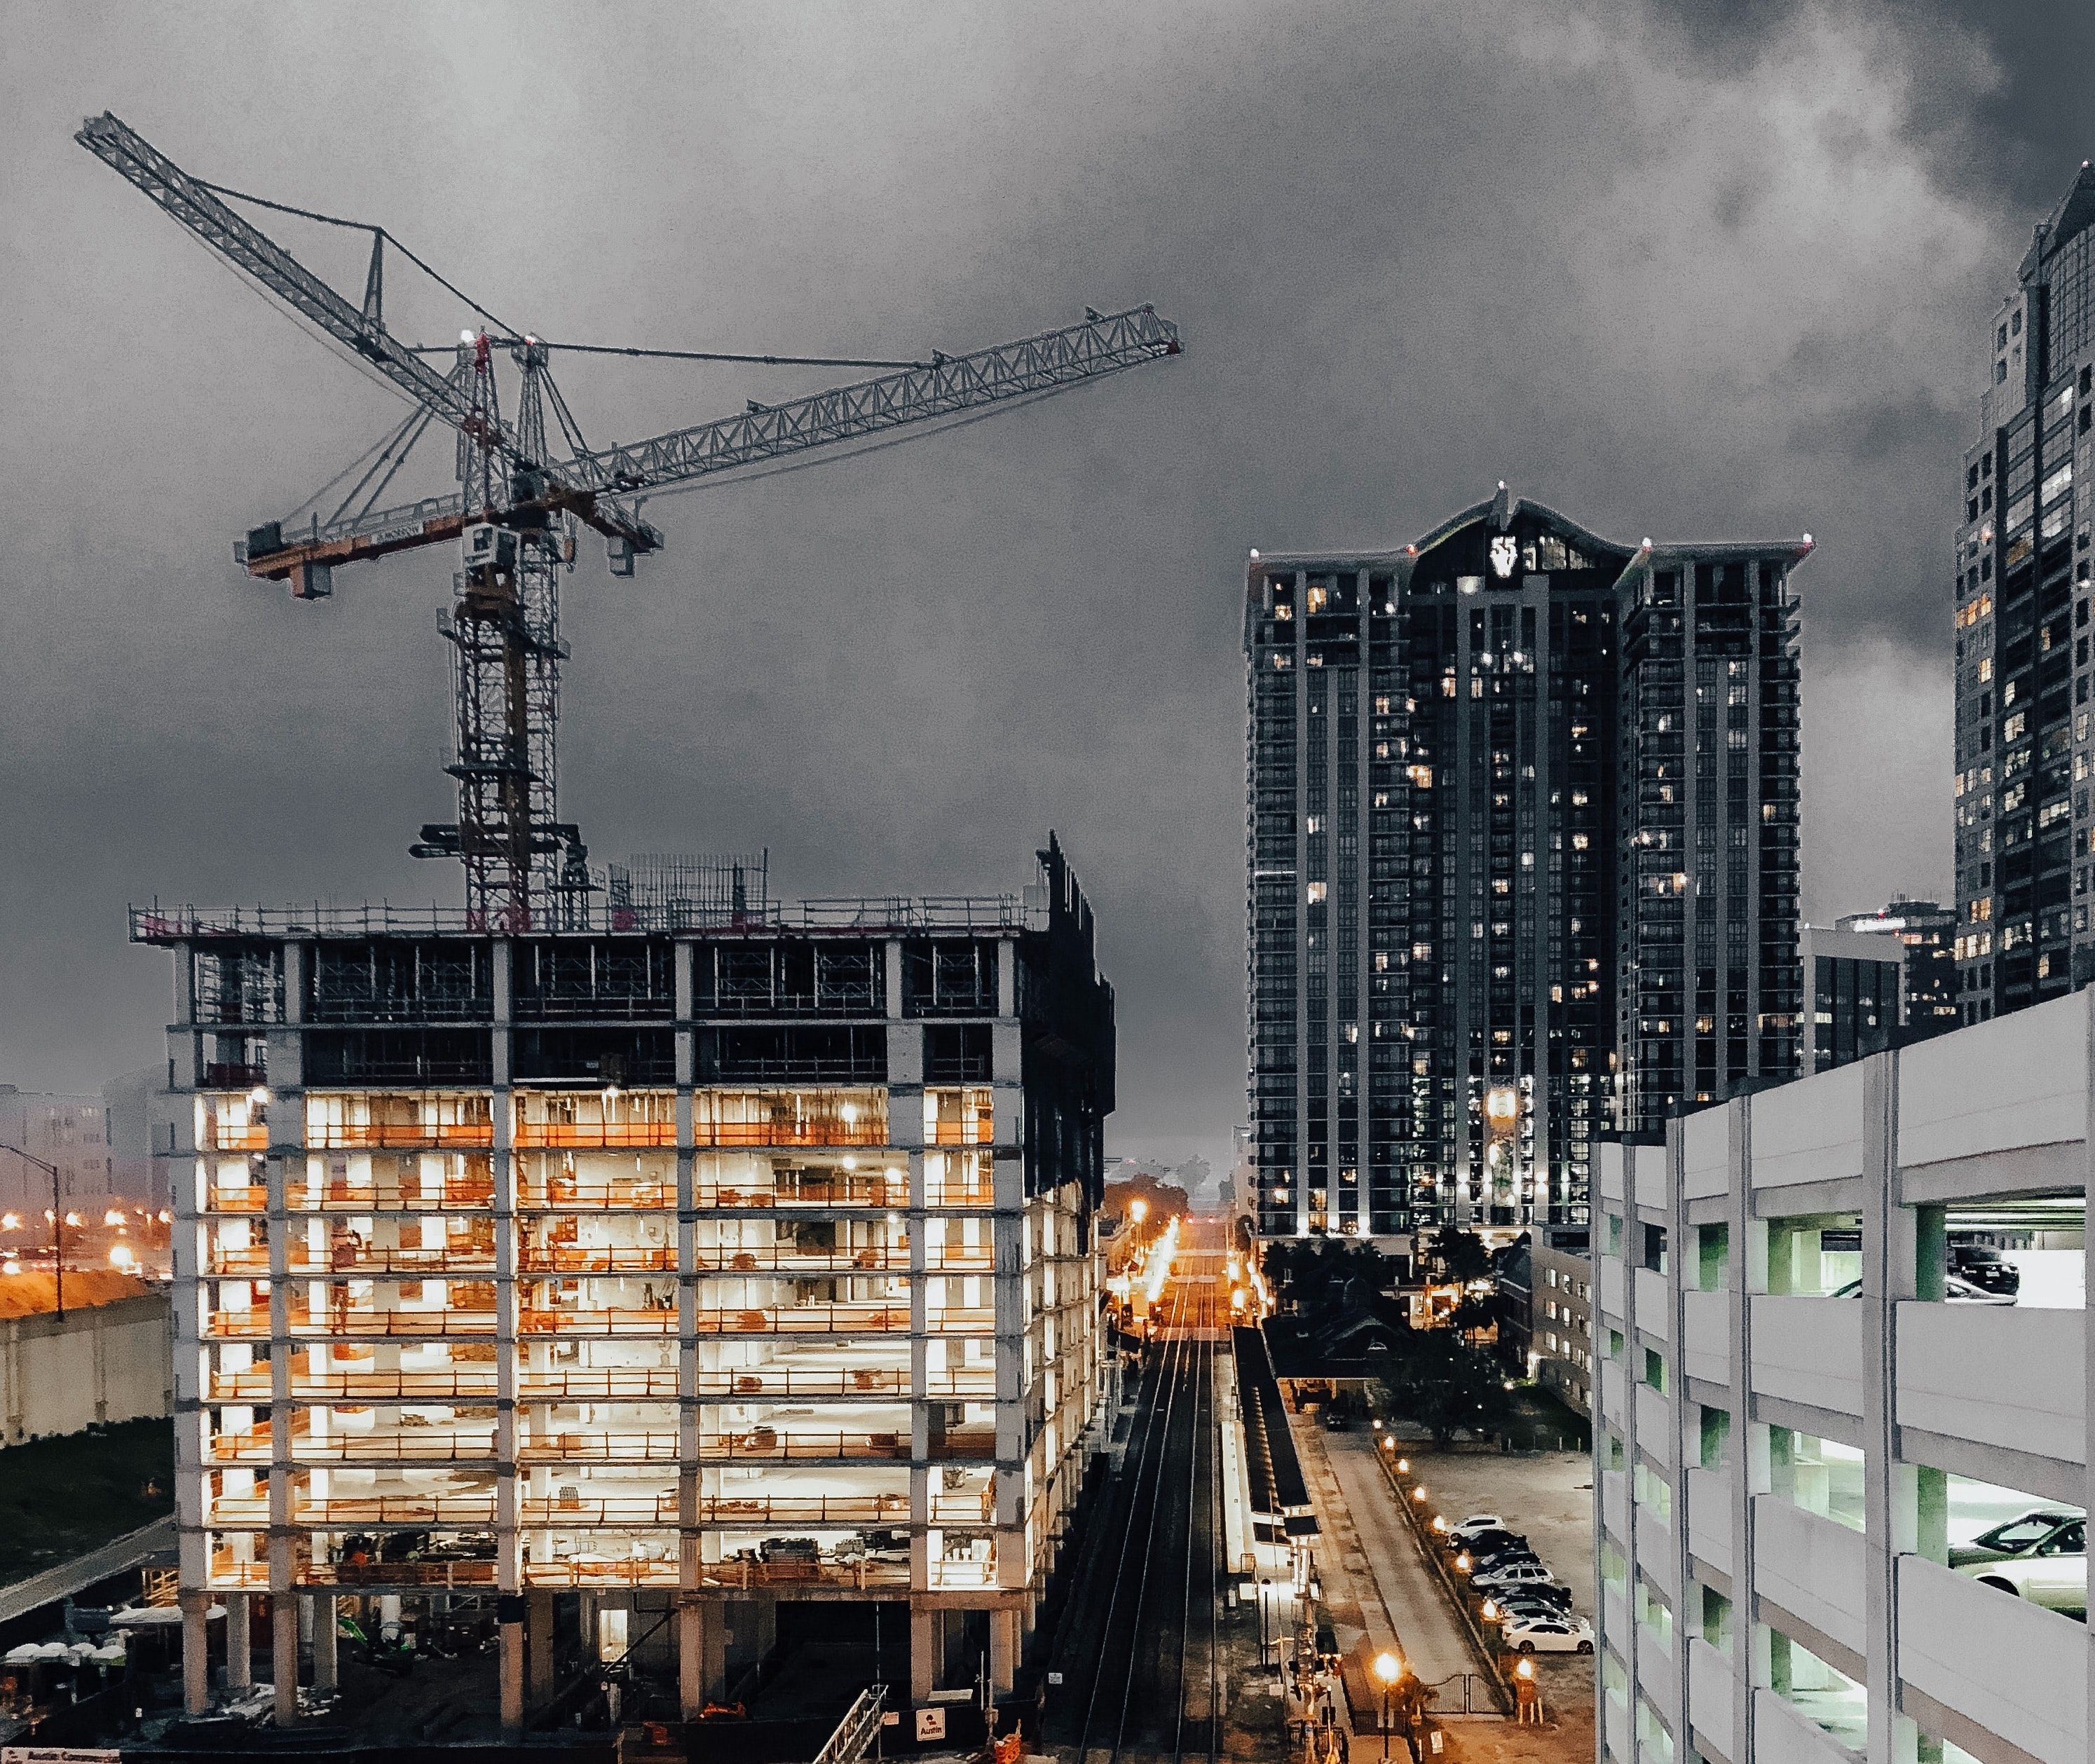
\includegraphics{img/crane.jpg} Photo by Nathan Waters on Unsplash

\end{footnotesize}}

\hypertarget{introduction}{%
\section{Introduction}\label{introduction}}

This is the first in a series of posts offering suggested strategies for
leveraging open source technologies to provide straight-forward
solutions to one of the central challenges in the practice of data
science, i.e.~how to effectively communicate analysis results to clients
and collaborators. The strategy is based on a set of open source tools.
The list of technologies (software stack) we suggest for employment is:
linux, R, Shiny, Docker, docker-compose, Git, and Caddy. In this post
we'll make use of two cloud services: Gitlab and Amazon Web Service
(AWS). Further posts will describe alternate services, e.g.~using the
low cost cloud service: Hetzner.

Also described in other posts, even more straightforward strategies that
avoid Gitlab and docker-compose. These alternative approaches provides a
simpler initial construction, but a more labor intensive updating
process.

This initial post provides a minimal, proof-of-concept example of how to
apply these technologies for hosting an interactive Shiny application.

In the following we start with a very simple, but hopefully still
useful, stand-alone Shiny app developed on our local workstation. Then
after some straightforward interfacing with the AWS environment, we push
the Shiny app into the cloud, and end up with a secure (encrypted and
authenticated) app running on a website with a custom domain name.

\hypertarget{methods}{%
\section{Methods}\label{methods}}

Start by creating a repository (repo) for the project. The best way to
do this is to initiate the repo on gitlab and then \texttt{clone} it to
your local workstation. In other words, log into gitlab and create a new
empty repo, call it \texttt{power1\_app}; then on your local workstation
navigate to your Shiny development directory, say
\texttt{\textasciitilde{}/prj}, and clone the \texttt{power1\_app} repo
from gitlab:

\begin{tcolorbox}[enhanced jigsaw, title=\textcolor{quarto-callout-note-color}{\faInfo}\hspace{0.5em}{Details for creating a gitlab repo follow:}, colback=white, arc=.35mm, leftrule=.75mm, titlerule=0mm, bottomtitle=1mm, opacityback=0, opacitybacktitle=0.6, breakable, left=2mm, toptitle=1mm, bottomrule=.15mm, rightrule=.15mm, toprule=.15mm, colbacktitle=quarto-callout-note-color!10!white, coltitle=black, colframe=quarto-callout-note-color-frame]

\begin{itemize}
\item
  login to \texttt{gitlab} (screenshot)
\item
  click on \texttt{New\ project}. Then in \texttt{repository\ name}
  field enter \texttt{power1\_app}.
\item
  make the repo private, we only want to share with our collaborator at
  this point).
\item
  leave \texttt{deployment\ target} empty.
\item
  create the repo. Click \texttt{Create\ project} blue button at the
  bottom of the page.
\item
  on your laptop cd to development repo, say \textasciitilde/prj and
  clone the gitlab repo:
\end{itemize}

\begin{Shaded}
\begin{Highlighting}[]
\FunctionTok{git}\NormalTok{ clone https://gitlab.com/rgt47/power1\_app.git}
\BuiltInTok{cd}\NormalTok{ power1\_app}
\FunctionTok{git}\NormalTok{ clone https://gitlab.com/rgt47/images.git}
\end{Highlighting}
\end{Shaded}

\end{tcolorbox}

\begin{marginfigure}

{\centering 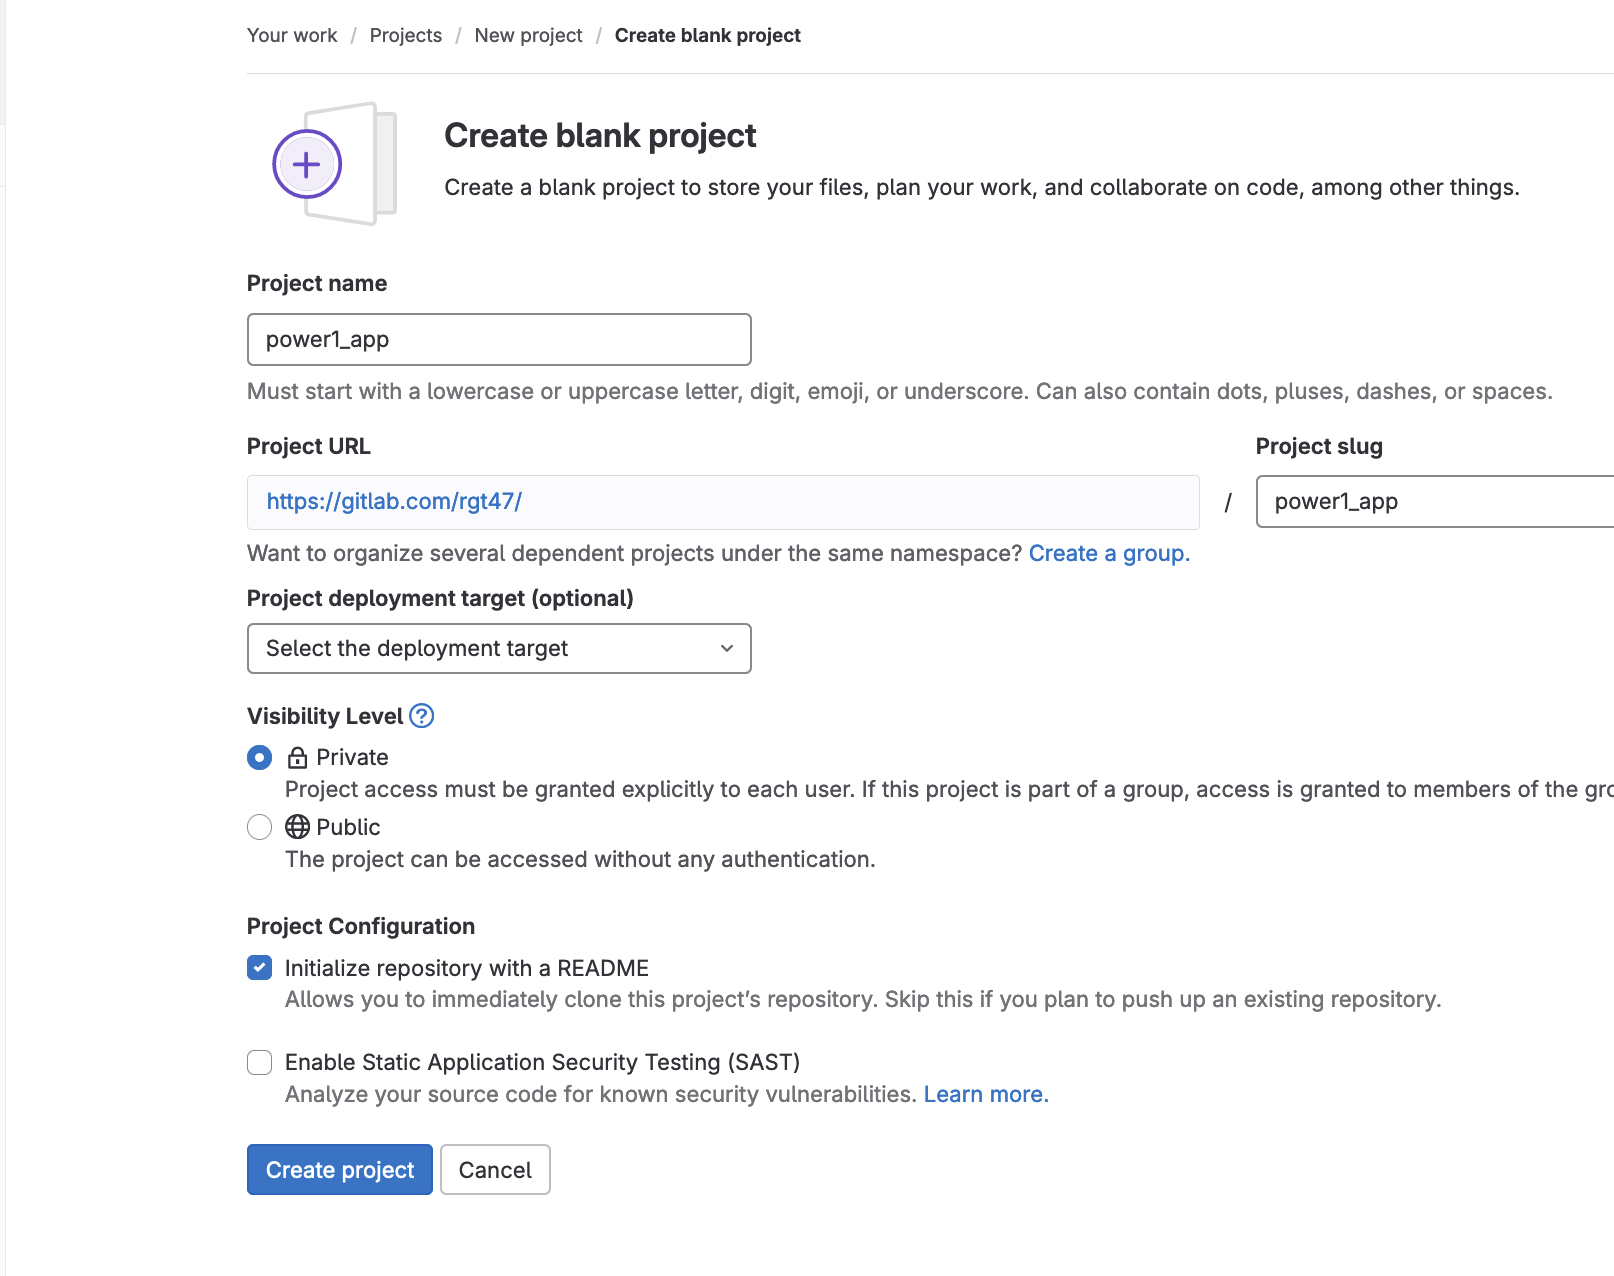
\includegraphics{img/gitlab1.png}

}

\end{marginfigure}

While in gitlab you should also create a second, public repo, call it
images. We'll use this repo to store screenshots of the app. After
cloning the repo to \textasciitilde/prj/power1\_app cd into the
directory and create two new sub-directories, \texttt{power1\_shiny} and
\texttt{site}. These directories will house our shiny app and our web
site landing page, respectively.

Lets jump ahead to the point where you've just finished developing a new
Shiny app named \texttt{app.R}, in the \texttt{power1\_shiny} directory.
(The methods described here apply generically to any Shiny app, but
we'll use one of our own for illustration). See the \texttt{R/Shiny}
code for our \texttt{power1\_shiny} app (\texttt{app.R}).

Consider an app that is a balance of simple and functional -- one that
calculates the power for a 2-sample t-test as a function of the
standardized effect size.

The app is minimal. Using only base R functions, with a minimum of
reactive widgets and layout commands to keep it simple while still
performing a useful function.

The code is here:

\begin{Shaded}
\begin{Highlighting}[]
\NormalTok{ui }\OtherTok{\textless{}{-}} \FunctionTok{fluidPage}\NormalTok{(}
\FunctionTok{titlePanel}\NormalTok{(}\StringTok{"Power Calculator for Two Group Parallel Designs"}\NormalTok{),}
\FunctionTok{sliderInput}\NormalTok{(}\StringTok{"N"}\NormalTok{, }\StringTok{"Total Sample Size:"}\NormalTok{, }\AttributeTok{min =} \DecValTok{0}\NormalTok{, }\AttributeTok{max =} \DecValTok{300}\NormalTok{, }\AttributeTok{value =} \DecValTok{100}\NormalTok{),}
\FunctionTok{plotOutput}\NormalTok{(}\StringTok{"plot"}\NormalTok{),}
\FunctionTok{verbatimTextOutput}\NormalTok{(}\StringTok{"eff"}\NormalTok{))}

\NormalTok{server }\OtherTok{\textless{}{-}} \ControlFlowTok{function}\NormalTok{(input, output, session) \{}
\NormalTok{  delta }\OtherTok{=} \FunctionTok{seq}\NormalTok{(}\DecValTok{0}\NormalTok{, }\FloatTok{1.5}\NormalTok{,.}\DecValTok{05}\NormalTok{)}
\NormalTok{  pow }\OtherTok{=} \FunctionTok{reactive}\NormalTok{(}\FunctionTok{sapply}\NormalTok{(delta, }\ControlFlowTok{function}\NormalTok{(x) }\FunctionTok{power.t.test}\NormalTok{(input}\SpecialCharTok{$}\NormalTok{N, }\AttributeTok{d=}\NormalTok{x)}\SpecialCharTok{$}\NormalTok{power ))}
\NormalTok{  eff }\OtherTok{=}  \FunctionTok{renderText}\NormalTok{(}\FunctionTok{power.t.test}\NormalTok{(input}\SpecialCharTok{$}\NormalTok{N, }\AttributeTok{power=}\NormalTok{.}\DecValTok{8}\NormalTok{)}\SpecialCharTok{$}\NormalTok{d)}
\NormalTok{  output}\SpecialCharTok{$}\NormalTok{plot }\OtherTok{\textless{}{-}} \FunctionTok{renderPlot}\NormalTok{(\{}
  \FunctionTok{plot}\NormalTok{(delta, }\FunctionTok{pow}\NormalTok{(), }\AttributeTok{cex=}\FloatTok{1.5}\NormalTok{, }\AttributeTok{ylab=}\StringTok{"power"}\NormalTok{)}
  \FunctionTok{abline}\NormalTok{(}\AttributeTok{h =}\NormalTok{ .}\DecValTok{8}\NormalTok{,  }\AttributeTok{col =} \StringTok{"red"}\NormalTok{, }\AttributeTok{lwd =}\FloatTok{2.5}\NormalTok{, }\AttributeTok{lty =} \DecValTok{4}\NormalTok{)}
  \FunctionTok{abline}\NormalTok{(}\AttributeTok{v =} \FunctionTok{eff}\NormalTok{(), }\AttributeTok{col =} \StringTok{"blue"}\NormalTok{,}\AttributeTok{lwd =}\FloatTok{2.5}\NormalTok{, }\AttributeTok{lty =} \DecValTok{4}\NormalTok{)\})  }
\NormalTok{  output}\SpecialCharTok{$}\NormalTok{eff }\OtherTok{\textless{}{-}} \FunctionTok{renderText}\NormalTok{(}
    \FunctionTok{paste0}\NormalTok{(}\StringTok{"Std. effect detectable with power 80\% = "}\NormalTok{, }\FunctionTok{eff}\NormalTok{()) )}
\NormalTok{\}}
\FunctionTok{shinyApp}\NormalTok{(ui, server)}
\end{Highlighting}
\end{Shaded}

We can test the app locally in our development directory,
\texttt{power1\_app}, by runnning it with the following command.

\begin{Shaded}
\begin{Highlighting}[]
\ExtensionTok{R} \AttributeTok{{-}e} \StringTok{"library(shiny); runApp(\textquotesingle{}power1\_shiny/app.R\textquotesingle{}, launch=T)"}
\end{Highlighting}
\end{Shaded}

This command will run the R program, load the Shiny package, and launch
the app in your default browser.

Figure 1 shows the Shiny app running locally in a browser, it consists
of a widget to select the sample size and provide a dynamic
visualization (2D plot) of the power as a function of the standardized
effect size:

\begin{marginfigure}

{\centering 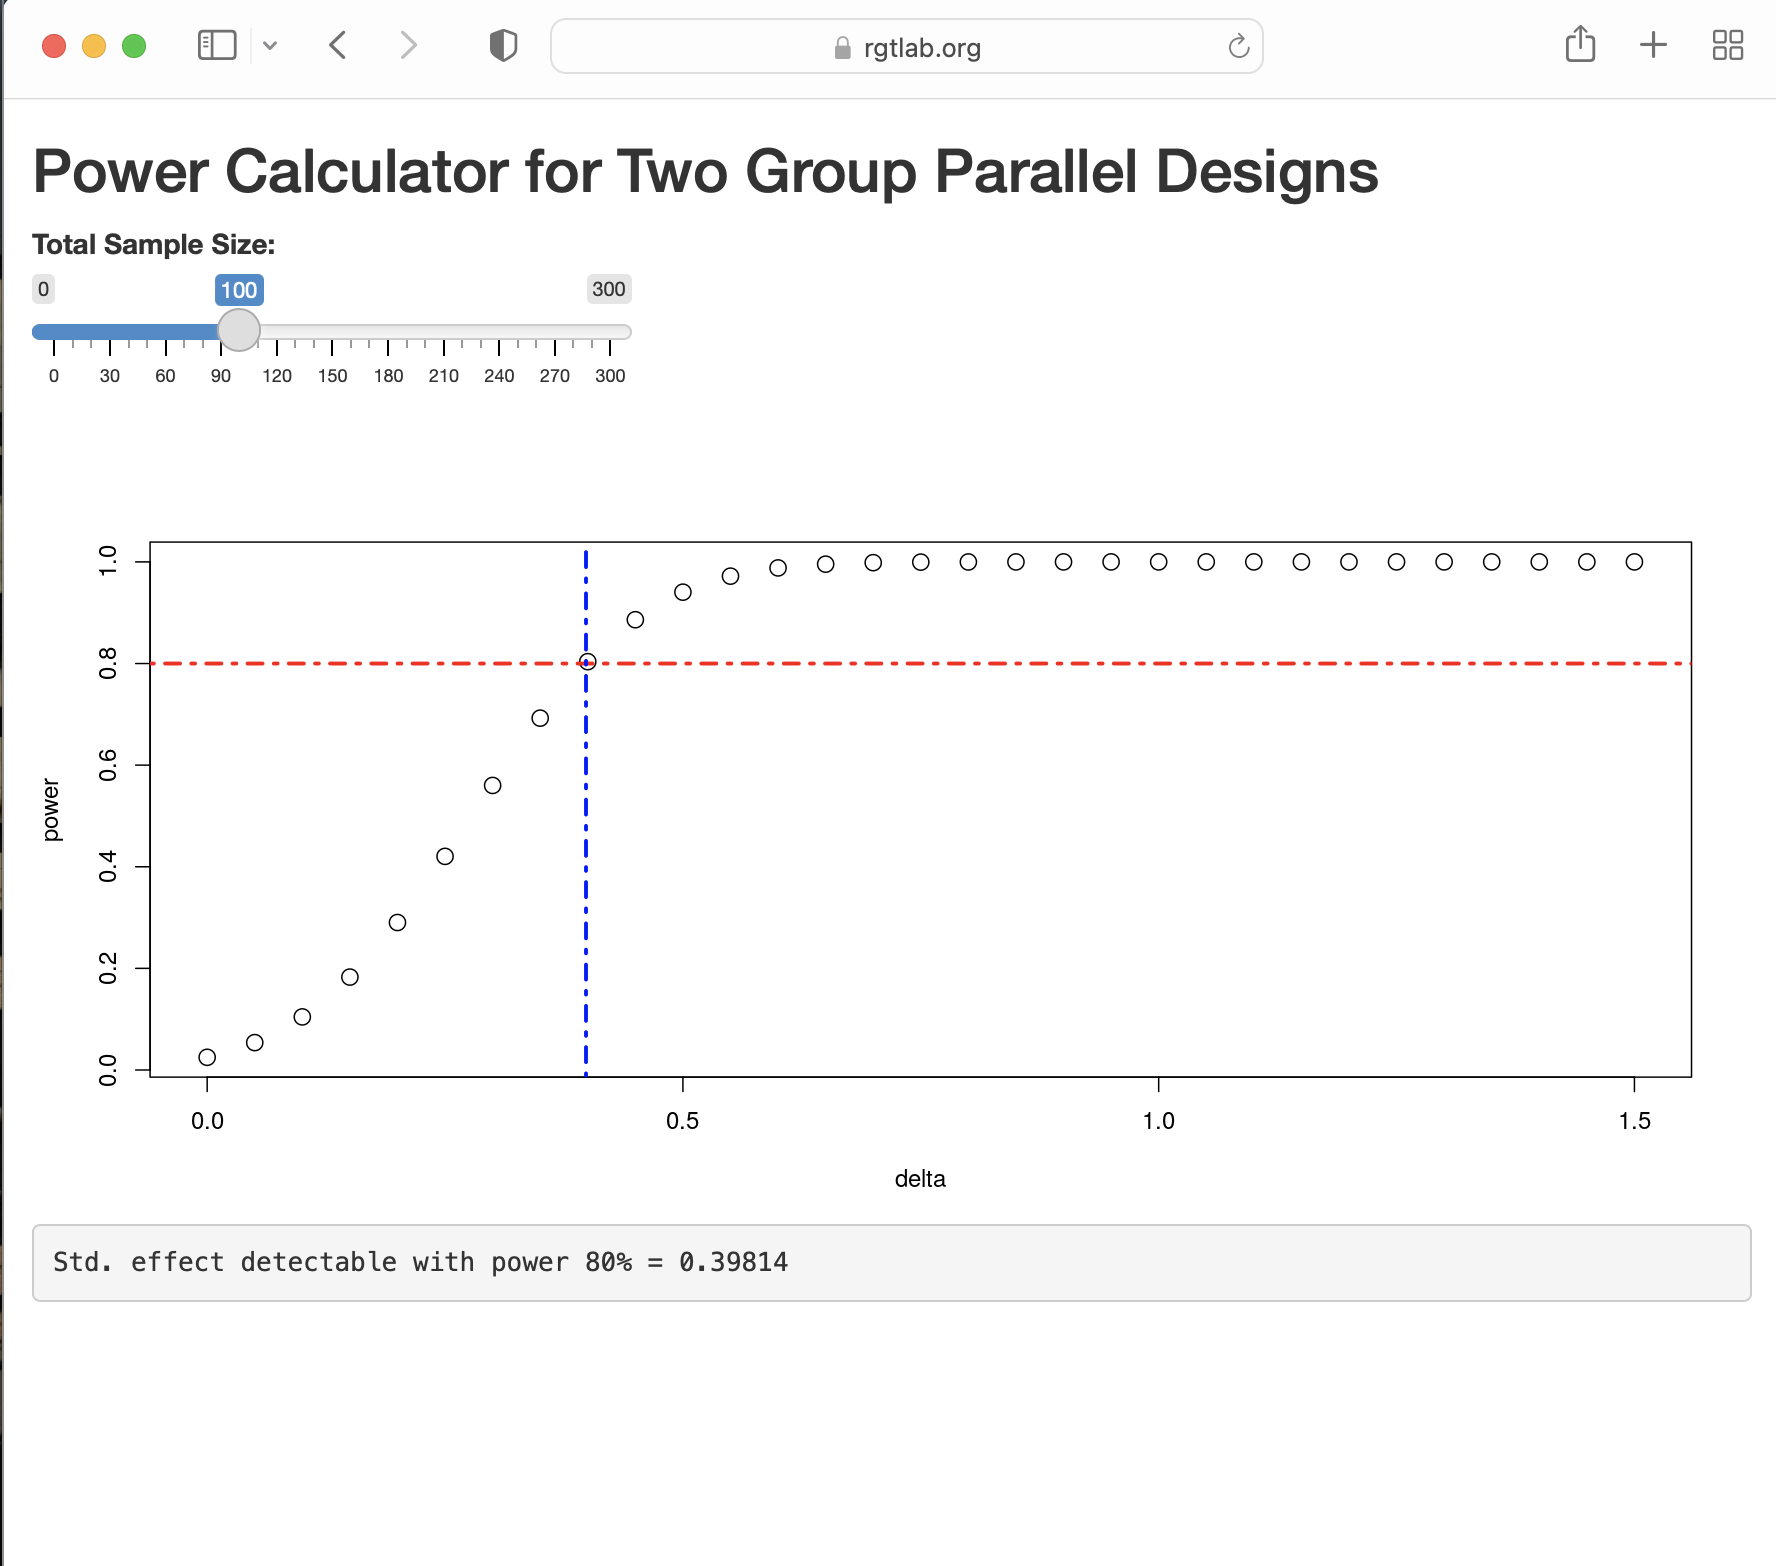
\includegraphics{img/shinyapppower1.png}

}

\caption{\emph{Shiny app}}

\end{marginfigure}

After we determine our app is working as designed, the next step is to
set up a secure hosting environment on a virtual server. Once the app is
hosted we simply need to send a link and security credentials to our
collaborators for them to have secure access to the Shiny app.

There are many ways to accomplish the hosting. Here we'll describe a
straightforward and efficient approach using mainstream cloud services
and open source tools. In other words, in the following we'll describe
how to `spin' up a virtual server on Amazon Web Service EC2 and in just
a few steps, through the application of Docker, R, Shiny, and Caddy
we'll have a fully functioning secure web app to share with our
colleagues.

\hypertarget{hosting}{%
\subsection{Hosting}\label{hosting}}

\begin{marginfigure}

{\centering 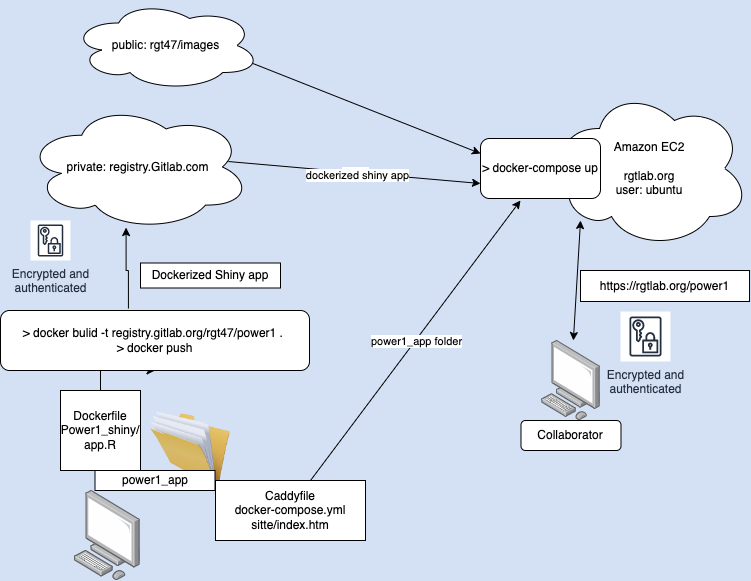
\includegraphics{img/compose_flow.png}

}

\caption{\emph{Data flow }}

\end{marginfigure}

Figure 2 illustrates the tools we'll use and the flow of program and
configuration files. In order to host \texttt{power1} online we'll need
to complete the following tasks:

\begin{enumerate}
\def\labelenumi{\arabic{enumi}.}
\tightlist
\item
  create a virtual server (connected via ssh) with a firewall
\item
  obtain a static IP address (to identify the server online)
\item
  obtain a domain name (name for IP address)
\item
  install and configure a webserver (tool to interact with https
  protocol requests and respond)
\item
  obtain and install an SSL certificate (to allow encrypted
  communication)
\item
  setup an authentication method (password protection)
\item
  configure a reverse proxy method (translate https, port 443, requests
  to Shiny, port 3838)
\end{enumerate}

At first glance these 7 requirements can appear daunting, but on closer
inspection all can be met with relative ease and minimal cost ( using a
cloud-hosting service, e.g.~Amazon's EC2 or Digital Ocean, and a
``leased'' domain name from, e.g.~GoDaddy, or Amazon's Route 53) or no
cost( if you have your own server with IP address, and domain name)

\hypertarget{select-a-hosting-service}{%
\subsection{Select a hosting service}\label{select-a-hosting-service}}

There are a number of cloud based server options: Microsoft Azure,
Oracle, Google Cloud, Amazon AWS EC2, Digital Ocean to name a few. Each
has their own approach to setting up a custom virtual server. Several
have free or low-cost service tiers available.

An overview of the process with EC2 follows. Detailed instructions for
AWS EC2 are covered in an earlier post
\href{https://focusonr.org/posts/setupaws/}{here}.

\begin{enumerate}
\def\labelenumi{\arabic{enumi}.}
\setcounter{enumi}{-1}
\tightlist
\item
  Create an account or sign in.
\item
  Set up an interactive environment with AWS server.

  \begin{enumerate}
  \def\labelenumii{\alph{enumii}.}
  \tightlist
  \item
    define ssh key-pair.
  \item
    configure firewall.
  \item
    request static IP.
  \item
    obtain domain name.
  \item
    select an instance and launch server.
  \end{enumerate}
\end{enumerate}

Once the server is available connect via ssh, and login,

The only necessary software to install is docker and git. Install both
with the following commands:

\begin{Shaded}
\begin{Highlighting}[]
\FunctionTok{sudo}\NormalTok{ apt install }\AttributeTok{{-}y}\NormalTok{ git}
\FunctionTok{sudo}\NormalTok{ snap install docker.io}
\end{Highlighting}
\end{Shaded}

Once the host is set up and the requisite software installed we'll have
a customized virtual server wtih a static IP address, and a unique
domain name and firewall in place. In other words, items 1, 2, and 3
from our \texttt{hosting} list above will be taken care of.

\hypertarget{website}{%
\subsection{Website}\label{website}}

To configure the web server and containerize our app we need to add
three files to the repo, to go along with our Shiny app.

We'll use a slightly indirect route to create and place the necessary
files on the server but this approach will allow to do all our
countinuing development on our local workstation and have the web app be
automatically continually undated. We'll create the configuration files
we need on our workstation and push them gitlab and from there they can
be accessed from our server.

These three configuation files are:

\hypertarget{docker}{%
\section{Docker}\label{docker}}

\begin{enumerate}
\def\labelenumi{\arabic{enumi}.}
\tightlist
\item
  a Docker configuration file (default name \texttt{Dockerfile})
\end{enumerate}

\marginnote{\begin{footnotesize}

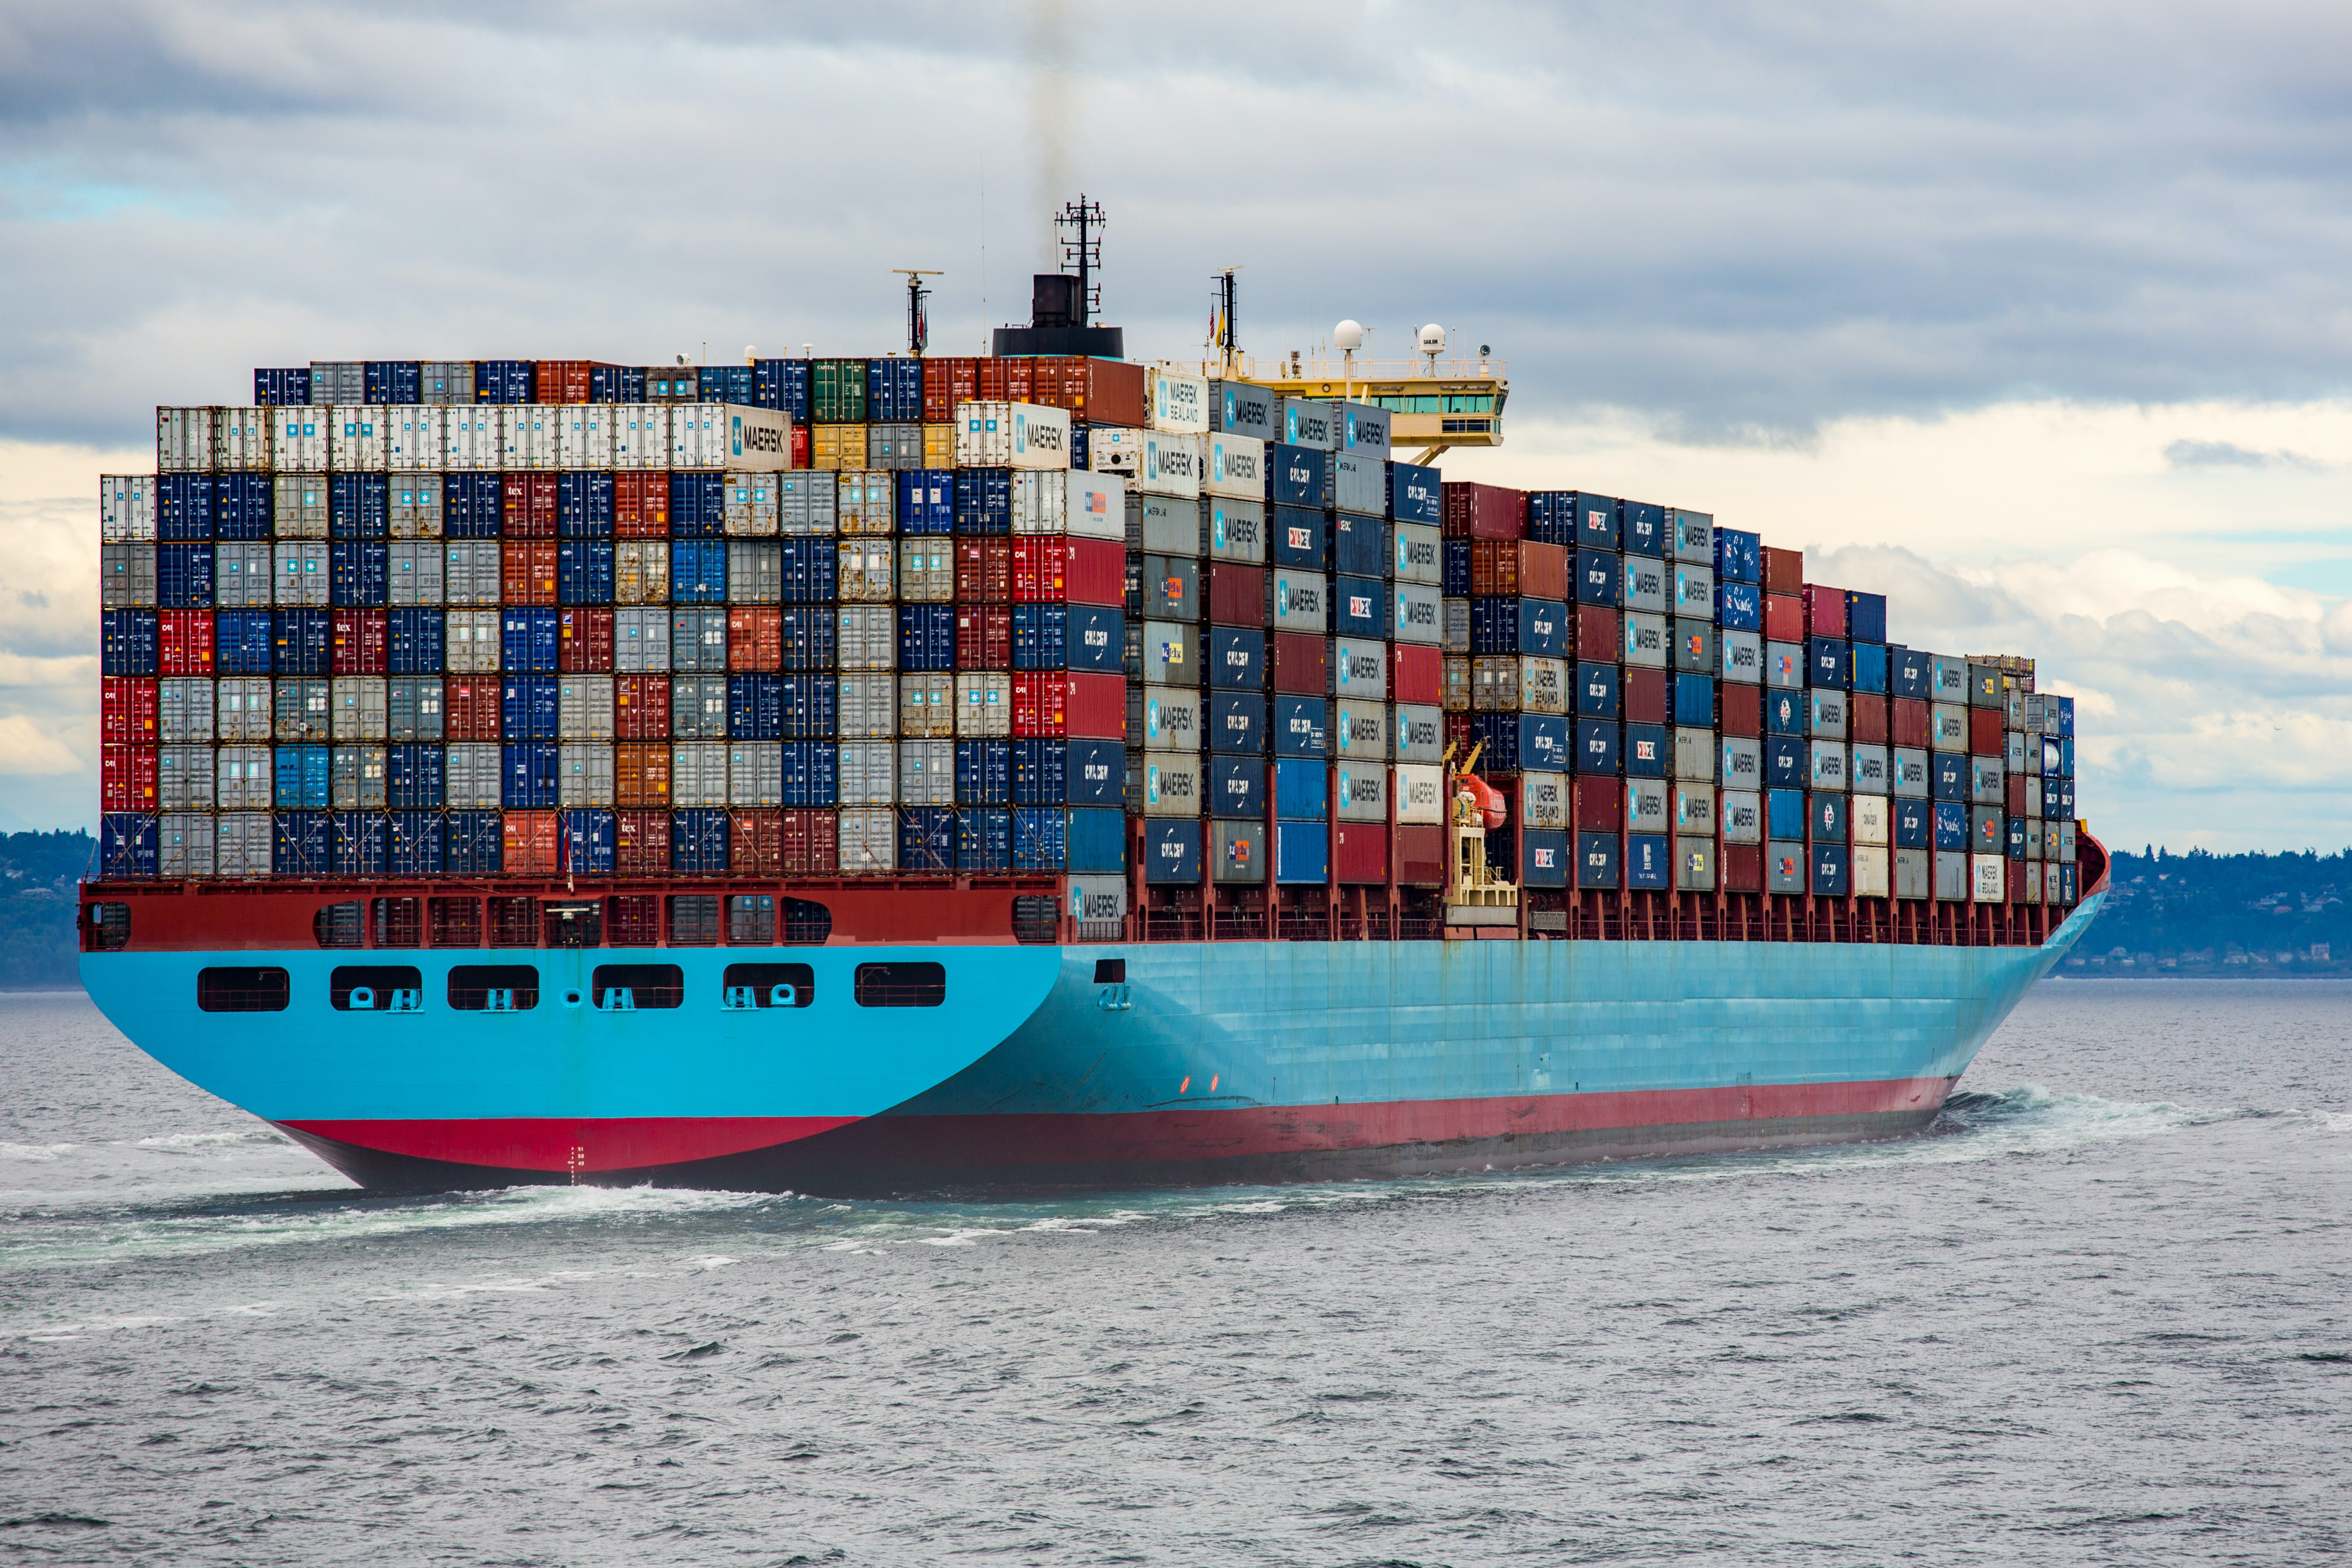
\includegraphics{img/docker1.jpg} Photo by Ian Taylor on Unsplash

\end{footnotesize}}

We'll use docker to access R/Shiny, and docker-compose to access Caddy,
our webserver. The first file is the dockerfile. Here is our minimal
dockerfile:

\begin{Shaded}
\begin{Highlighting}[]
\NormalTok{FROM rocker}\SpecialCharTok{/}\NormalTok{shiny}\SpecialCharTok{:}\DecValTok{4}\NormalTok{.}\FloatTok{2.0}
\NormalTok{RUN rm }\SpecialCharTok{{-}}\NormalTok{rf }\SpecialCharTok{/}\NormalTok{srv}\SpecialCharTok{/}\NormalTok{shiny}\SpecialCharTok{{-}}\NormalTok{server}
\NormalTok{COPY }\SpecialCharTok{/}\NormalTok{power1\_shiny}\SpecialCharTok{/}\ErrorTok{*} \ErrorTok{/}\NormalTok{srv}\SpecialCharTok{/}\NormalTok{shiny}\SpecialCharTok{{-}}\NormalTok{server}\SpecialCharTok{/}
\NormalTok{USER shiny}
\NormalTok{CMD [}\StringTok{"/usr/bin/shiny{-}server"}\NormalTok{]}
\end{Highlighting}
\end{Shaded}

{\marginnote{\begin{footnotesize}Note: We placed the
\texttt{power1\_shiny/app.R} code in the default location
\texttt{/srv/shiny-server} so we only need to start the Shiny server and
it will find the shiny program\end{footnotesize}}}

This configuration file instructs Docker to build a container based on a
Rocker/Shiny image (which itself is a ubuntu image with R and Shiny
installed) then copy into the container the \texttt{power1\_shiny.R}
code and finally launch Shiny on (default) port 3838. We placed the
app.R code in the default location \texttt{/srv/shiny-server} we only
need to start the server and it will find the shiny program.

Then build and push the image to the \texttt{gitlab} container registry.

\begin{Shaded}
\begin{Highlighting}[]
\ExtensionTok{docker}\NormalTok{ build }\AttributeTok{{-}t}\NormalTok{ registry.gitlab.com/rgt47/power1\_app/power1\_image:v1.0 }\DataTypeTok{\textbackslash{}}
        \AttributeTok{{-}{-}platform}\NormalTok{ linux/x86\_64 .}
\ExtensionTok{docker}\NormalTok{ push registry.gitlab.com/rgt47/power1\_app/power1\_image:v1.0}
\end{Highlighting}
\end{Shaded}

\begin{enumerate}
\def\labelenumi{\arabic{enumi}.}
\setcounter{enumi}{1}
\tightlist
\item
  a Caddy web server configuration file (default name
  \texttt{Caddyfile})
\end{enumerate}

We'll use \texttt{Caddy} as our web server. Caddy is an open-source tool
that has the very useful feature of automating the acquisition and
installing of an SSL certificate. An SSL cert is required by most
browsers to use the encrypted communication protocol https.

We use the caddy configuration file to specify three critical things.

\begin{enumerate}
\def\labelenumi{\arabic{enumi}.}
\tightlist
\item
  the site domain name.
\item
  the `reverse proxy' map that redirects requests to port 443 (ssl port)
  to port 3838 (Shiny port).
\item
  add login credentials for all users (e.g.~bob/vanilla47):
\end{enumerate}

\hypertarget{caddy}{%
\section{Caddy}\label{caddy}}

Our barebones \texttt{Caddyfile} looks like this:

\begin{Shaded}
\begin{Highlighting}[]
\CommentTok{\# use caddy auth tool to generate a password via the \textasciigrave{}bcrypt\textasciigrave{} algorithm. }
\CommentTok{\# \textgreater{} caddy hash{-}password {-}{-}plaintext hiccup }

\NormalTok{rgtlab.org \{}
\NormalTok{basicauth }\SpecialCharTok{/}\NormalTok{power1}\SpecialCharTok{/}\ErrorTok{*}\NormalTok{ \{}
\NormalTok{    Bob }\SpecialCharTok{$}\NormalTok{2a}\SpecialCharTok{$}\DecValTok{14}\SpecialCharTok{$}\NormalTok{Zkx19XLiW6VYouLHR5NmfOFU0z2GTNmpkT}\SpecialCharTok{/}\NormalTok{5qqR7hx4IjWJPDhjvG}
\NormalTok{\}}
\NormalTok{    root }\SpecialCharTok{*} \ErrorTok{/}\NormalTok{srv}
\NormalTok{    handle\_path }\SpecialCharTok{/}\NormalTok{power1}\SpecialCharTok{/}\ErrorTok{*}\NormalTok{ \{}
\NormalTok{        reverse\_proxy power1}\SpecialCharTok{:}\DecValTok{3838}
\NormalTok{    \}}
\NormalTok{    file\_server}
\NormalTok{\}}
\end{Highlighting}
\end{Shaded}

We can accomplish what we need for items 4, 5, and 7 through the
Caddyfile.

Note:

\begin{itemize}
\tightlist
\item
  rgtlab.org is our domain name
\item
  \texttt{handle\_path} maps all https requests to port 3838 where Shiny
  is listening.
\end{itemize}

Providing our servers domain name, \texttt{rgtlab.org} is sufficient to
initiate an exchange with the \texttt{letsencrypt} service to generates
an SSL certificate.

And a third file is a config file for Docker Compose. Docker Compose is
a Docker module that provides a framework for running multi-container
applications. This docker compose YAML file instructs Docker to
containerize our Shiny app, pull a caddy webserver image from Docker Hub
and create a local network for the two containers to communicate in.

\begin{enumerate}
\def\labelenumi{\arabic{enumi}.}
\setcounter{enumi}{2}
\tightlist
\item
  a Docker-compose configuration file (default name
  \texttt{docker-compose.yml}).
\end{enumerate}

The docker-compose.yml file:

\begin{Shaded}
\begin{Highlighting}[]
\NormalTok{version}\SpecialCharTok{:} \StringTok{"3.7"}

\NormalTok{services}\SpecialCharTok{:}
\NormalTok{  power1}\SpecialCharTok{:}
\NormalTok{    image}\SpecialCharTok{:}\NormalTok{ registry.gitlab.com}\SpecialCharTok{/}\NormalTok{rgt47}\SpecialCharTok{/}\NormalTok{power1\_app}\SpecialCharTok{/}\NormalTok{power1\_image}\SpecialCharTok{:}\NormalTok{v1}\FloatTok{.0}
\NormalTok{    restart}\SpecialCharTok{:}\NormalTok{ unless}\SpecialCharTok{{-}}\NormalTok{stopped}
\NormalTok{    expose}\SpecialCharTok{:}
      \SpecialCharTok{{-}} \StringTok{"3838"}
\NormalTok{  caddy}\SpecialCharTok{:}
\NormalTok{    image}\SpecialCharTok{:}\NormalTok{ caddy}\SpecialCharTok{:}\DecValTok{2}\NormalTok{.}\FloatTok{6.4}\SpecialCharTok{{-}}\NormalTok{alpine}
\NormalTok{    restart}\SpecialCharTok{:}\NormalTok{ always}
\NormalTok{    ports}\SpecialCharTok{:}
      \SpecialCharTok{{-}} \StringTok{"443:443"}
\NormalTok{    volumes}\SpecialCharTok{:}
      \SpecialCharTok{{-}} \ErrorTok{$}\NormalTok{PWD}\SpecialCharTok{/}\NormalTok{Caddyfile}\SpecialCharTok{:}\ErrorTok{/}\NormalTok{etc}\SpecialCharTok{/}\NormalTok{caddy}\SpecialCharTok{/}\NormalTok{Caddyfile}
      \SpecialCharTok{{-}} \ErrorTok{$}\NormalTok{PWD}\SpecialCharTok{/}\NormalTok{site}\SpecialCharTok{:}\ErrorTok{/}\NormalTok{srv}
      \SpecialCharTok{{-}}\NormalTok{ caddy\_data}\SpecialCharTok{:}\ErrorTok{/}\NormalTok{data}
      \SpecialCharTok{{-}}\NormalTok{ caddy\_config}\SpecialCharTok{:}\ErrorTok{/}\NormalTok{config}
\NormalTok{    depends\_on}\SpecialCharTok{:}
      \SpecialCharTok{{-}}\NormalTok{ power1}
\NormalTok{    environment}\SpecialCharTok{:}
      \SpecialCharTok{{-}}\NormalTok{ HOST}\OtherTok{=}\StringTok{"rgtlab.org"}
      \SpecialCharTok{{-}}\NormalTok{ EMAIL}\OtherTok{=}\StringTok{"rgthomas@ucsd.edu"}
\NormalTok{volumes}\SpecialCharTok{:}
\NormalTok{  caddy\_data}\SpecialCharTok{:}
\NormalTok{  caddy\_config}\SpecialCharTok{:}
\end{Highlighting}
\end{Shaded}

\hypertarget{landing-page}{%
\section{Landing Page}\label{landing-page}}

Lastly, we need an html file, \texttt{index.html} in a subdirectory
named \texttt{site} that provides the landing page for our server.

\begin{Shaded}
\begin{Highlighting}[]
\SpecialCharTok{\textless{}!}\NormalTok{DOCTYPE html}\SpecialCharTok{\textgreater{}}
\ErrorTok{\textless{}}\NormalTok{html}\SpecialCharTok{\textgreater{}}
  \ErrorTok{\textless{}}\NormalTok{head}\SpecialCharTok{\textgreater{}}
    \ErrorTok{\textless{}}\NormalTok{meta charset}\OtherTok{=}\StringTok{"utf{-}8"}\SpecialCharTok{\textgreater{}}
    \ErrorTok{\textless{}}\NormalTok{meta http}\SpecialCharTok{{-}}\NormalTok{equiv}\OtherTok{=}\StringTok{"X{-}UA{-}Compatible"}\NormalTok{ content}\OtherTok{=}\StringTok{"IE=edge"}\SpecialCharTok{\textgreater{}}
    \ErrorTok{\textless{}}\NormalTok{meta name}\OtherTok{=}\StringTok{"viewport"}\NormalTok{ content}\OtherTok{=}\StringTok{"width=device{-}width, initial{-}scale=1"}\SpecialCharTok{\textgreater{}}
    \ErrorTok{\textless{}}\NormalTok{title}\SpecialCharTok{\textgreater{}}\NormalTok{Power Calculators}\SpecialCharTok{\textless{}}\ErrorTok{/}\NormalTok{title}\SpecialCharTok{\textgreater{}}
    \ErrorTok{\textless{}}\NormalTok{link rel}\OtherTok{=}\StringTok{"stylesheet"}\NormalTok{ href}\OtherTok{=}\StringTok{"https://unpkg.com/bulma@0.9.0/css/bulma.min.css"} \SpecialCharTok{/}\ErrorTok{\textgreater{}}
  \ErrorTok{\textless{}/}\NormalTok{head}\SpecialCharTok{\textgreater{}}
  \ErrorTok{\textless{}}\NormalTok{body}\SpecialCharTok{\textgreater{}}
    \ErrorTok{\textless{}}\NormalTok{div id}\OtherTok{=}\StringTok{"app"}\SpecialCharTok{\textgreater{}}
      \ErrorTok{\textless{}}\NormalTok{section class}\OtherTok{=}\StringTok{"hero is{-}small"}\SpecialCharTok{\textgreater{}}
        \ErrorTok{\textless{}}\NormalTok{div class}\OtherTok{=}\StringTok{"hero{-}body"}\SpecialCharTok{\textgreater{}}
          \ErrorTok{\textless{}}\NormalTok{div class}\OtherTok{=}\StringTok{"container has{-}text{-}centered"}\SpecialCharTok{\textgreater{}}
            \ErrorTok{\textless{}}\NormalTok{h1 class}\OtherTok{=}\StringTok{"title"}\SpecialCharTok{\textgreater{}}\NormalTok{RGT Lab Power Calculators}\SpecialCharTok{\textless{}}\ErrorTok{/}\NormalTok{h1}\SpecialCharTok{\textgreater{}}
          \ErrorTok{\textless{}/}\NormalTok{div}\SpecialCharTok{\textgreater{}}
        \ErrorTok{\textless{}/}\NormalTok{div}\SpecialCharTok{\textgreater{}}
      \ErrorTok{\textless{}/}\NormalTok{section}\SpecialCharTok{\textgreater{}}
            \ErrorTok{\textless{}}\NormalTok{hr}\SpecialCharTok{\textgreater{}}

            \ErrorTok{\textless{}}\NormalTok{div class}\OtherTok{=}\StringTok{"columns"}\SpecialCharTok{\textgreater{}}
              \ErrorTok{\textless{}}\NormalTok{div class}\OtherTok{=}\StringTok{"column is{-}4 is{-}offset{-}1"}\SpecialCharTok{\textgreater{}}
      \ErrorTok{\textless{}}\NormalTok{img src}\OtherTok{=}\StringTok{"https://github.com/rgt47/power0/blob/master/power1.png?raw=true"}
\NormalTok{        width}\OtherTok{=}\StringTok{"200"}\NormalTok{ height}\OtherTok{=}\StringTok{"250"}\NormalTok{  ”float}\SpecialCharTok{:}\NormalTok{ left; padding}\SpecialCharTok{:}\NormalTok{ 3px 3px 0px 3px;” }\SpecialCharTok{\textgreater{}}
              \ErrorTok{\textless{}/}\NormalTok{div}\SpecialCharTok{\textgreater{}}
              \ErrorTok{\textless{}}\NormalTok{div class}\OtherTok{=}\StringTok{"column is{-}6"}\SpecialCharTok{\textgreater{}}
                \ErrorTok{\textless{}}\NormalTok{h1 class}\OtherTok{=}\StringTok{"title"}\SpecialCharTok{\textgreater{}}\NormalTok{ Power1 App }\SpecialCharTok{\textless{}}\ErrorTok{/}\NormalTok{h1}\SpecialCharTok{\textgreater{}}
                \ErrorTok{\textless{}}\NormalTok{p}\SpecialCharTok{\textgreater{}}\NormalTok{ Power }\ControlFlowTok{for}\NormalTok{ two}\SpecialCharTok{{-}}\NormalTok{sample t}\SpecialCharTok{{-}}\NormalTok{test }\SpecialCharTok{\textless{}}\ErrorTok{/}\NormalTok{p}\SpecialCharTok{\textgreater{}}
                \ErrorTok{\textless{}}\NormalTok{br}\SpecialCharTok{\textgreater{}}
                \ErrorTok{\textless{}}\NormalTok{a href}\OtherTok{=}\StringTok{"./power1/"}\NormalTok{ class}\OtherTok{=}\StringTok{"button is{-}info"}\SpecialCharTok{\textgreater{}}\NormalTok{Go to app}\SpecialCharTok{\textless{}}\ErrorTok{/}\NormalTok{a}\SpecialCharTok{\textgreater{}}
              \ErrorTok{\textless{}/}\NormalTok{div}\SpecialCharTok{\textgreater{}}
            \ErrorTok{\textless{}/}\NormalTok{div}\SpecialCharTok{\textgreater{}}

    \ErrorTok{\textless{}/}\NormalTok{div}\SpecialCharTok{\textgreater{}}
  \ErrorTok{\textless{}/}\NormalTok{body}\SpecialCharTok{\textgreater{}}
\ErrorTok{\textless{}/}\NormalTok{html}\SpecialCharTok{\textgreater{}}
\end{Highlighting}
\end{Shaded}

At this point our \texttt{power1\_app} repo looks like this:

\begin{Shaded}
\begin{Highlighting}[]
\NormalTok{.}
\NormalTok{├── Caddyfile}
\NormalTok{├── Dockerfile}
\NormalTok{├── docker{-}compose.yml}
\NormalTok{└── site}
\NormalTok{    └── index.html}
\end{Highlighting}
\end{Shaded}

\hypertarget{gitlab}{%
\section{gitlab}\label{gitlab}}

Push the new content to gitlab.

\begin{Shaded}
\begin{Highlighting}[]
\FunctionTok{git}\NormalTok{ push}
\end{Highlighting}
\end{Shaded}

Next login to the virtual server and clone the repo from gitlab.

\begin{Shaded}
\begin{Highlighting}[]
\FunctionTok{ssh}\NormalTok{ rgtlab.org}
\FunctionTok{git}\NormalTok{ clone https://gitlab.com/rgt47/power1\_app.git}
\end{Highlighting}
\end{Shaded}

Lastly, cd into \texttt{power1\_app} directory and run

\begin{Shaded}
\begin{Highlighting}[]
\ExtensionTok{docker}\NormalTok{ compose up }\AttributeTok{{-}d}
\end{Highlighting}
\end{Shaded}

and you're good to go! The power1\_shiny app is available at

\begin{Shaded}
\begin{Highlighting}[]
\ExtensionTok{https://rgtlab.org/}
\end{Highlighting}
\end{Shaded}

\hypertarget{appendices}{%
\section{Appendices}\label{appendices}}

\hypertarget{tip-1.-docker-on-m1-macbook.}{%
\subsection{Tip 1. Docker on M1
macbook.}\label{tip-1.-docker-on-m1-macbook.}}

To get docker functioning properly with \texttt{rocker} images on M1 Mac
desktop use \texttt{-\/-platform} option.

\begin{Shaded}
\begin{Highlighting}[]
\ExtensionTok{docker}\NormalTok{ build }\AttributeTok{{-}t}\NormalTok{ power1\_shiny }\AttributeTok{{-}{-}platform}\NormalTok{ linux/x86\_64 .}
\ExtensionTok{docker}\NormalTok{ run }\AttributeTok{{-}d} \AttributeTok{{-}p}\NormalTok{ 80:3838 }\AttributeTok{{-}{-}platform}\NormalTok{ linux/x86\_64 power1\_shiny}
\end{Highlighting}
\end{Shaded}

\hypertarget{tip-2-add-user-to-docker-group-on-server.}{%
\subsection{Tip 2 add user to docker group on
server.}\label{tip-2-add-user-to-docker-group-on-server.}}

Add ubuntu to the docker group to allow docker to run without sudo.

\begin{Shaded}
\begin{Highlighting}[]
\FunctionTok{sudo}\NormalTok{ usermod }\AttributeTok{{-}aG}\NormalTok{ docker }\VariableTok{$\{USER\}}
\end{Highlighting}
\end{Shaded}

\hypertarget{tip-3-ssh-config-file.}{%
\subsection{Tip 3 ssh config file.}\label{tip-3-ssh-config-file.}}

For convenience, construct a \texttt{config} file in
\texttt{\textasciitilde{}/.ssh} as:

\begin{Shaded}
\begin{Highlighting}[]



\ExtensionTok{Host}\NormalTok{ rgtlab.org}
\ExtensionTok{HostName}\NormalTok{ 13.57.139.31 }\CommentTok{\# static IP}
\ExtensionTok{User}\NormalTok{ ubuntu }\CommentTok{\# default user on ubuntu server}
\ExtensionTok{Port}\NormalTok{ 22  }\CommentTok{\# the default port ssh uses}
\ExtensionTok{IdentityFile}\NormalTok{ \textasciitilde{}/.ssh/power1\_app.pem}
\end{Highlighting}
\end{Shaded}

then you can ssh into the new server with

\begin{Shaded}
\begin{Highlighting}[]
\FunctionTok{sh}\OperatorTok{\textgreater{}}\NormalTok{ ssh rgtlab.org }
\end{Highlighting}
\end{Shaded}

\hypertarget{references}{%
\section{References}\label{references}}

\begin{itemize}
\tightlist
\item
  \href{https://focusonr.org/posts/server_setup_aws_console/}{Focus on
  R: a new qblog - Set up a virtual server on AWS (in anticipation of
  hosting Shiny apps)}
\item
  \href{https://focusonr.org/posts/server_setup_aws_cli/}{Focus on R: a
  new qblog - Set up a virtual server on AWS with AWS CLI}
\item
  \href{https://hosting.analythium.io/shiny-apps-with-docker-compose-part-1-development/}{Shiny
  Apps with Docker Compose, Part 1: Development}
\item
  \href{https://hosting.analythium.io/shiny-apps-with-docker-compose-part-2-production/}{Shiny
  Apps with Docker Compose, Part 2: Production}
\end{itemize}

\hypertarget{appendix}{%
\section{APPENDIX}\label{appendix}}

\begin{Shaded}
\begin{Highlighting}[]

\OperatorTok{\textgreater{}}\NormalTok{ cd }\ExtensionTok{/Users/zenn/Dropbox/prj/c060}
\OperatorTok{\textgreater{}}\NormalTok{ aws\_create\_keypair.sh }\ExtensionTok{power1\_app}
\OperatorTok{\textgreater{}}\NormalTok{ aws\_create\_security\_group.sh }\ExtensionTok{{-}s}\NormalTok{ power1\_app }\AttributeTok{{-}h}\NormalTok{ on }\AttributeTok{{-}k}\NormalTok{ on }\AttributeTok{{-}i}\NormalTok{ on }\AttributeTok{{-}j}\NormalTok{ on}
\OperatorTok{\textgreater{}}\NormalTok{ security\_grp=}\StringTok{"sg{-}0679282d70f727f1e"}
\OperatorTok{\textgreater{}}\NormalTok{ echo }\VariableTok{$security\_grp}
\ExtensionTok{If}\NormalTok{ we need a new IP address:}
\OperatorTok{\textgreater{}}\NormalTok{ static\_ip=}\KeywordTok{\textasciigrave{}}\ExtensionTok{aws}\NormalTok{ ec2 allocate{-}address }\KeywordTok{|} \ExtensionTok{jq} \AttributeTok{{-}r} \StringTok{\textquotesingle{}.PublicIp\textquotesingle{}}\KeywordTok{\textasciigrave{}}
\OperatorTok{\textgreater{}}\NormalTok{ echo }\VariableTok{$static\_ip}
\OperatorTok{\textgreater{}}\NormalTok{ aws\_create\_instance.sh }\ExtensionTok{{-}p}\NormalTok{ power1\_app}
\VariableTok{instance\_id}\OperatorTok{=}\StringTok{"i{-}0ecb046262ab6efca"}
 \ExtensionTok{aws}\NormalTok{ ec2 associate{-}address }\AttributeTok{{-}{-}instance{-}id} \VariableTok{$instance\_id} \AttributeTok{{-}{-}public{-}ip} \VariableTok{$static\_ip}

\ExtensionTok{associate}\NormalTok{ IP with domain name in Route 53}
\ExtensionTok{change}\NormalTok{ the IP address in \textasciitilde{}/.ssh/config}

\FunctionTok{scp} \AttributeTok{{-}i} \StringTok{"\textasciitilde{}/.ssh/power1\_app.pem"}\NormalTok{ .zshrc ubuntu@rgtlab.org:\textasciitilde{}}
\FunctionTok{scp} \AttributeTok{{-}i} \StringTok{"\textasciitilde{}/.ssh/power1\_app.pem"}\NormalTok{ .vimrc ubuntu@rgtlab.org:\textasciitilde{}}

\OperatorTok{\textgreater{}}\NormalTok{ ssh }\ExtensionTok{rgtlab.org}

\ExtensionTok{Check}\NormalTok{ the log of your user data script in:}
    \ExtensionTok{/var/log/cloud{-}init{-}output.log}

\FunctionTok{git}\NormalTok{ clone https://gitlab.com/rgt47/power1\_app.git}
\FunctionTok{git}\NormalTok{ clone https://gitlab.com/rgt47/images.git}

 \ExtensionTok{docker}\NormalTok{ run }\AttributeTok{{-}d} \DataTypeTok{\textbackslash{}}
    \AttributeTok{{-}{-}name}\OperatorTok{=}\NormalTok{hello }\DataTypeTok{\textbackslash{}}
    \AttributeTok{{-}{-}restart}\OperatorTok{=}\NormalTok{always }\DataTypeTok{\textbackslash{}}
    \AttributeTok{{-}p}\NormalTok{ 9000:3838 }\DataTypeTok{\textbackslash{}}
\NormalTok{    registry.gitlab.com/analythium/shinyproxy{-}hello/hello:latest}


 \ExtensionTok{docker}\NormalTok{ run }\AttributeTok{{-}d} \DataTypeTok{\textbackslash{}}
    \AttributeTok{{-}{-}name}\OperatorTok{=}\NormalTok{power1 }\DataTypeTok{\textbackslash{}}
    \AttributeTok{{-}{-}restart}\OperatorTok{=}\NormalTok{always }\DataTypeTok{\textbackslash{}}
    \AttributeTok{{-}p}\NormalTok{ 9001:3838 }\DataTypeTok{\textbackslash{}}
\NormalTok{    registry.gitlab.com/rgt47/power1\_app/power1\_image:v1.0}

\ExtensionTok{http://rgtlab.org:9001/}
\ExtensionTok{displays}\NormalTok{ power1\_shiny app }

\FunctionTok{git}\NormalTok{ clone https://github.com/analythium/docker{-}compose{-}shiny{-}example.git}
\BuiltInTok{cd}\NormalTok{ docker{-}compose{-}shiny{-}example.git}

\ExtensionTok{edit}\NormalTok{ the docker{-}compose{-}prod.yml file to include domain name and email}

\ExtensionTok{docker}\NormalTok{ compose }\DataTypeTok{\textbackslash{}}
  \AttributeTok{{-}f}\NormalTok{ docker{-}compose.yml }\DataTypeTok{\textbackslash{}}
  \AttributeTok{{-}f}\NormalTok{ docker{-}compose{-}prod.yml }\DataTypeTok{\textbackslash{}}
\NormalTok{  up }\AttributeTok{{-}d}

\ExtensionTok{change}\NormalTok{ docker{-}compose.yml to point at gitlab repo rgt47/power1\_app for }\StringTok{\textquotesingle{}hello\textquotesingle{}}\NormalTok{ app}

\ExtensionTok{works.}

\ExtensionTok{now}\NormalTok{ cp  docker{-}compose{-}shiny{-}example.git}
\ExtensionTok{to} \StringTok{\textquotesingle{}master\textquotesingle{}}\NormalTok{ and begin to transform }\StringTok{\textquotesingle{}master\textquotesingle{}}\NormalTok{ into }\StringTok{\textquotesingle{}power1\_app\textquotesingle{}}
\ExtensionTok{keep}\NormalTok{ logging info}

\ExtensionTok{to}\NormalTok{ rebuild all the containers in the docker{-}compose.yml file:}

\ExtensionTok{docker}\NormalTok{ compose up }\AttributeTok{{-}{-}build} \AttributeTok{{-}d} 

\ExtensionTok{remove}\NormalTok{ all containers and images }

\ExtensionTok{docker}\NormalTok{ system prune }\AttributeTok{{-}a}

\ControlFlowTok{if} \ExtensionTok{changes}\NormalTok{ are made to shiny app on m1 mac. stop the compose network, pull updated container and restart.}

\BuiltInTok{cd}\NormalTok{ power1\_shiny}
\ExtensionTok{vim}\NormalTok{ app.R}
\BuiltInTok{cd}\NormalTok{ \textasciitilde{}/Dropbox/prj/c060/docker\_simple\_power1\_app}
\ExtensionTok{docker}\NormalTok{ build }\AttributeTok{{-}t}\NormalTok{ registry.gitlab.com/rgt47/power1\_app/power1\_image:v1.0 }\AttributeTok{{-}{-}platform}\NormalTok{ linux/x86\_64 .}
\ExtensionTok{docker}\NormalTok{ push registry.gitlab.com/rgt47/power1\_app/power1\_image:v1.0}

\ExtensionTok{docker}\NormalTok{ compose stop}
\ExtensionTok{docker}\NormalTok{ compose rm }\AttributeTok{{-}f}
\ExtensionTok{docker}\NormalTok{ compose pull   }
\ExtensionTok{docker}\NormalTok{ compose up }\AttributeTok{{-}d}


\ExtensionTok{\textasciitilde{}/master{-}repo} \ErrorTok{(}\ExtensionTok{main}\NormalTok{ ✘}\KeywordTok{)}\ExtensionTok{✖✹}\NormalTok{ ᐅ cat Caddyfile}
\ExtensionTok{rgtlab.org}\NormalTok{ \{}
\ExtensionTok{basicauth}\NormalTok{ /power1/}\PreprocessorTok{*}\NormalTok{ \{}
    \ExtensionTok{Bob} \VariableTok{$2}\NormalTok{a}\VariableTok{$1}\NormalTok{4}\VariableTok{$Zkx19XLiW6VYouLHR5NmfOFU0z2GTNmpkT}\NormalTok{/5qqR7hx4IjWJPDhjvG}
\ErrorTok{\}}

    \ExtensionTok{root} \PreprocessorTok{*}\NormalTok{ /srv}
    \ExtensionTok{handle\_path}\NormalTok{ /power1/}\PreprocessorTok{*}\NormalTok{ \{}
        \ExtensionTok{reverse\_proxy}\NormalTok{ power1:3838}
    \ErrorTok{\}}
    \ExtensionTok{file\_server}
\ErrorTok{\}}


\ExtensionTok{version:} \StringTok{"3.7"}

\ExtensionTok{services:}
  \ExtensionTok{power1:}
    \ExtensionTok{image:}\NormalTok{ registry.gitlab.com/rgt47/power1\_app/power1\_image:v1.0}
    \ExtensionTok{restart:}\NormalTok{ unless{-}stopped}
    \ExtensionTok{expose:}
      \ExtensionTok{{-}} \StringTok{"3838"}
  \ExtensionTok{caddy:}
    \ExtensionTok{image:}\NormalTok{ caddy:2.6.4{-}alpine}
    \ExtensionTok{restart:}\NormalTok{ always}
    \ExtensionTok{ports:}
      \ExtensionTok{{-}} \StringTok{"443:443"}
    \ExtensionTok{volumes:}
      \ExtensionTok{{-}} \VariableTok{$PWD}\NormalTok{/Caddyfile:/etc/caddy/Caddyfile}
      \ExtensionTok{{-}} \VariableTok{$PWD}\NormalTok{/site:/srv}
      \ExtensionTok{{-}}\NormalTok{ caddy\_data:/data}
      \ExtensionTok{{-}}\NormalTok{ caddy\_config:/config}
    \ExtensionTok{depends\_on:}
      \ExtensionTok{{-}}\NormalTok{ power1}
    \ExtensionTok{environment:}
      \ExtensionTok{{-}}\NormalTok{ HOST=}\StringTok{"rgtlab.org"}
      \ExtensionTok{{-}}\NormalTok{ EMAIL=}\StringTok{"rgthomas@ucsd.edu"}
\ExtensionTok{volumes:}
  \ExtensionTok{caddy\_data:}
  \ExtensionTok{caddy\_config:}

\ExtensionTok{\textasciitilde{}/master{-}repo} \ErrorTok{(}\ExtensionTok{main}\NormalTok{ ✘}\KeywordTok{)}\ExtensionTok{✖✹}\NormalTok{ ᐅ cat site/index.html}
\OperatorTok{\textless{}}\NormalTok{!DOCTYPE }\ExtensionTok{html}\OperatorTok{\textgreater{}}
\OperatorTok{\textless{}}\NormalTok{html}\OperatorTok{\textgreater{}}
  \OperatorTok{\textless{}}\NormalTok{head}\OperatorTok{\textgreater{}}
    \OperatorTok{\textless{}}\NormalTok{meta }\VariableTok{charset}\OperatorTok{=}\StringTok{"utf{-}8"}\OperatorTok{\textgreater{}}
    \OperatorTok{\textless{}}\NormalTok{meta }\ExtensionTok{http{-}equiv=}\StringTok{"X{-}UA{-}Compatible"}\NormalTok{ content=}\StringTok{"IE=edge"}\OperatorTok{\textgreater{}}
    \OperatorTok{\textless{}}\NormalTok{meta }\VariableTok{name}\OperatorTok{=}\StringTok{"viewport"} \VariableTok{content}\OperatorTok{=}\StringTok{"width=device{-}width, initial{-}scale=1"}\OperatorTok{\textgreater{}}
    \OperatorTok{\textless{}}\NormalTok{title}\OperatorTok{\textgreater{}}\NormalTok{Power }\ExtensionTok{Calculators}\OperatorTok{\textless{}}\NormalTok{/title}\OperatorTok{\textgreater{}}
    \OperatorTok{\textless{}}\NormalTok{link }\VariableTok{rel}\OperatorTok{=}\StringTok{"stylesheet"} \VariableTok{href}\OperatorTok{=}\StringTok{"https://unpkg.com/bulma@0.9.0/css/bulma.min.css"} \ExtensionTok{/}\OperatorTok{\textgreater{}}
  \OperatorTok{\textless{}}\NormalTok{/head}\OperatorTok{\textgreater{}}
  \OperatorTok{\textless{}}\NormalTok{body}\OperatorTok{\textgreater{}}
    \OperatorTok{\textless{}}\NormalTok{div }\VariableTok{id}\OperatorTok{=}\StringTok{"app"}\OperatorTok{\textgreater{}}
      \OperatorTok{\textless{}}\NormalTok{section }\VariableTok{class}\OperatorTok{=}\StringTok{"hero is{-}small"}\OperatorTok{\textgreater{}}
        \OperatorTok{\textless{}}\NormalTok{div }\VariableTok{class}\OperatorTok{=}\StringTok{"hero{-}body"}\OperatorTok{\textgreater{}}
          \OperatorTok{\textless{}}\NormalTok{div }\VariableTok{class}\OperatorTok{=}\StringTok{"container has{-}text{-}centered"}\OperatorTok{\textgreater{}}
            \OperatorTok{\textless{}}\NormalTok{h1 }\VariableTok{class}\OperatorTok{=}\StringTok{"title"}\OperatorTok{\textgreater{}}\NormalTok{RGT }\ExtensionTok{Lab}\NormalTok{ Power Calculators}\OperatorTok{\textless{}}\NormalTok{/h1}\OperatorTok{\textgreater{}}
          \OperatorTok{\textless{}}\NormalTok{/div}\OperatorTok{\textgreater{}}
        \OperatorTok{\textless{}}\NormalTok{/div}\OperatorTok{\textgreater{}}
      \OperatorTok{\textless{}}\NormalTok{/section}\OperatorTok{\textgreater{}}
            \OperatorTok{\textless{}}\NormalTok{hr}\OperatorTok{\textgreater{}}

            \OperatorTok{\textless{}}\NormalTok{div }\VariableTok{class}\OperatorTok{=}\StringTok{"columns"}\OperatorTok{\textgreater{}}
              \OperatorTok{\textless{}}\NormalTok{div }\VariableTok{class}\OperatorTok{=}\StringTok{"column is{-}4 is{-}offset{-}1"}\OperatorTok{\textgreater{}}
      \OperatorTok{\textless{}}\NormalTok{img }\VariableTok{src}\OperatorTok{=}\StringTok{"https://github.com/rgt47/power0/blob/master/power1.png?raw=true"}
        \VariableTok{width}\OperatorTok{=}\StringTok{"200"} \VariableTok{height}\OperatorTok{=}\StringTok{"250"}  \ExtensionTok{”float:}\NormalTok{ left}\KeywordTok{;} \ExtensionTok{padding:}\NormalTok{ 3px 3px 0px 3px}\KeywordTok{;}\ExtensionTok{”} \OperatorTok{\textgreater{}}
              \OperatorTok{\textless{}}\NormalTok{/div}\OperatorTok{\textgreater{}}
              \OperatorTok{\textless{}}\NormalTok{div }\VariableTok{class}\OperatorTok{=}\StringTok{"column is{-}6"}\OperatorTok{\textgreater{}}
                \OperatorTok{\textless{}}\NormalTok{h1 }\VariableTok{class}\OperatorTok{=}\StringTok{"title"}\OperatorTok{\textgreater{}}\NormalTok{ Power1 }\ExtensionTok{App} \OperatorTok{\textless{}}\NormalTok{/h1}\OperatorTok{\textgreater{}}
                \OperatorTok{\textless{}}\NormalTok{p}\OperatorTok{\textgreater{}}\NormalTok{ Power }\ControlFlowTok{for}\NormalTok{ two}\ExtensionTok{{-}sample}\NormalTok{ t{-}test }\OperatorTok{\textless{}}\NormalTok{/p}\OperatorTok{\textgreater{}}
                \OperatorTok{\textless{}}\NormalTok{br}\OperatorTok{\textgreater{}}
                \OperatorTok{\textless{}}\NormalTok{a }\VariableTok{href}\OperatorTok{=}\StringTok{"./power1/"} \VariableTok{class}\OperatorTok{=}\StringTok{"button is{-}info"}\OperatorTok{\textgreater{}}\NormalTok{Go }\ExtensionTok{to}\NormalTok{ app}\OperatorTok{\textless{}}\NormalTok{/a}\OperatorTok{\textgreater{}}
              \OperatorTok{\textless{}}\NormalTok{/div}\OperatorTok{\textgreater{}}
            \OperatorTok{\textless{}}\NormalTok{/div}\OperatorTok{\textgreater{}}


    \OperatorTok{\textless{}}\NormalTok{/div}\OperatorTok{\textgreater{}}
  \OperatorTok{\textless{}}\NormalTok{/body}\OperatorTok{\textgreater{}}
\OperatorTok{\textless{}}\NormalTok{/html}\OperatorTok{\textgreater{}}


\end{Highlighting}
\end{Shaded}




\end{document}
